%Schriftgröße, Layout, Papierformat, Art des Dokumentes
\documentclass[12pt,oneside,a4paper,bibliography=totoc, listof=totoc,]{scrartcl}


\usepackage[utf8]{inputenc}
%Einstellungen der Seitenränder
\usepackage[left=3.0cm,right=2.0cm,top=2.5cm,bottom=2cm,includeheadfoot]{geometry}
%neue Rechtschreibung
\usepackage{ngerman}
%Kopf- und Fußzeile
\usepackage{fancyhdr}
%Quellen
\usepackage{cite}
%URLs
\usepackage{url}
%Grafik umbruch
\usepackage{wrapfig}
% Kein Textumbruch
%\usepackage[none]{hyphenat} 
%\sloppy   
% Kopf & Fusszeilen
\pagestyle{fancy}
\fancyhf{}  
% irgendwas
\usepackage{setspace}
%Warnings
\setkomafont{descriptionlabel}{\rmfamily\bfseries}
%Kein Abstand unter / über Bildern
\setlength{\intextsep}{5mm plus3mm minus2mm}
%Kopfzeile links bzw. innen
\fancyhead[L]{Andreas Knöpfle, Mathias Hodler}
%Kopfzeile rechts bzw. außen
\fancyhead[R]{Dokumentation iPad Spot The Difference}
%Linie oben
\renewcommand{\headrulewidth}{0.5pt}
%Zeilenabstand
\renewcommand{\baselinestretch}{1.50}\normalsize
% Aufnahme in das Inhaltsverzeichnis 
\setcounter{tocdepth}{4}
%Nummerierung vertiefen
\setcounter{secnumdepth}{4}
%caption
\usepackage[tableposition=top]{caption}
\captionsetup{font={small}}

%bilder floattext
\usepackage{float} 
\usepackage{subfigure} 
\usepackage{floatflt}

\usepackage{picins}

\newenvironment{Itemize}[1][1]
  {\begingroup\setstretch{#1}\vspace{-.5\baselineskip}\itemize}
  {\enditemize\endgroup}

%\renewcommand{\sectionmark}[1]{\markright{#1}{}}
%Fußzeile
\renewcommand{\sectionmark}[1]{\markboth{\thesection\ #1}{}}
\renewcommand{\subsectionmark}[1]{\markright{\thesubsection\ #1}}


\newcommand{\beginToEnd}{1. September 2009 bis 28. Februar 2010}
%Fußzeile rechts bzw. außen
\fancyfoot[C]{\thepage}
\fancyfoot[R]{\leftmark}
%Linie unten
\renewcommand{\footrulewidth}{0.5pt}
\usepackage[pdftex]{graphicx}
\usepackage{acronym}


%Abkürzungen Kursiv
\renewcommand*{\acsfont}[1]{\textit{#1}}
\renewcommand*{\acffont}[1]{\textit{#1}}

%Quellenvz Name
\renewcommand{\refname}{Literatur und Quellenverzeichnis}
%Paragrapheneinschub verhindern
 \setlength{\parindent}{0pt} 
\begin{document}

\thispagestyle{empty}

\begin{center}
	\vskip 1.5cm
	\begin{center}
		
\includegraphics[width=30mm]{bilder/htwg-logo}
	\end{center}	
	\vskip 0.8cm

	\LARGE \textbf{Dokumentation iPad Spot The Difference}

	\vskip 0.1cm
	\LARGE \textbf{Objective-C/Cocoa Vorlesung} 
	\vskip 1cm	
	
	\large{  
  	\vskip 1cm
   	
	Bericht von\\
	\textbf{Andreas Knöpfle (281187)\\ Mathias Hodler(281159)}

	\vskip 1.0cm
	
	Konstanz, \today}
	
	
\end{center}

\clearpage

\tableofcontents
\newpage
	
	\section{Abkürzungsverzeichniss} 
		\begin{acronym}
 			\acro{JPEG}{Joint Photographic Experts Group, ein im Web weit verbreitetes Grafikformat für verlustbehaftete oder verlustfreie Kompression von digitalen Fotografien.}
 			\acro{IOS}{ein Betriebssystem der Firma Apple für mobile Geräte. Es basiert auf Mac OS X und ist das Standard-Betriebssystem der Apple-Produkte iPhone, iPod touch, iPad und der zweiten Generation des Apple TV}
		\end{acronym}
	\newpage		
	
		
	\section{Idee und Spielkonzept}
		 
		\newpage
	\section{Spezifikation}
		 	
		\newpage
	\section{Umsetzung}
		 	
		\newpage	
	\section{Lösung}
		Im folgenden Abschnitt sind die Lösungen zu den Rätseln abgebildet.


  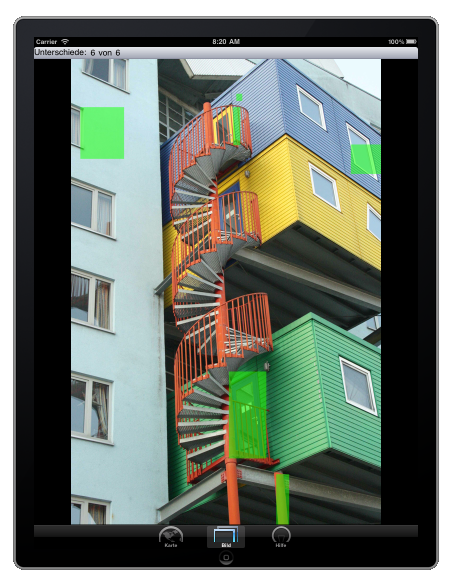
\includegraphics[width=1.0\textwidth]{bilder/loesung1.png}
  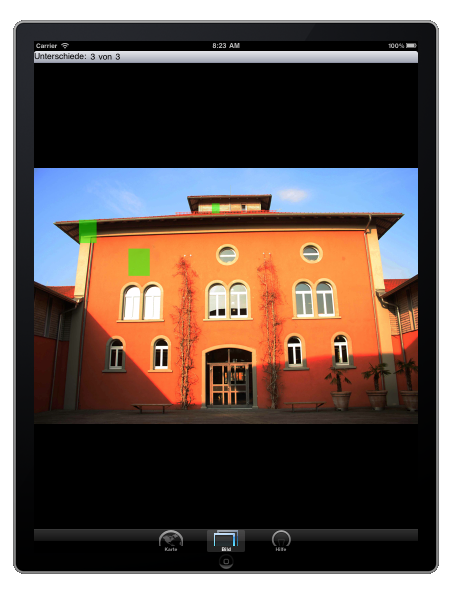
\includegraphics[width=1.0\textwidth]{bilder/loesung2.png}
  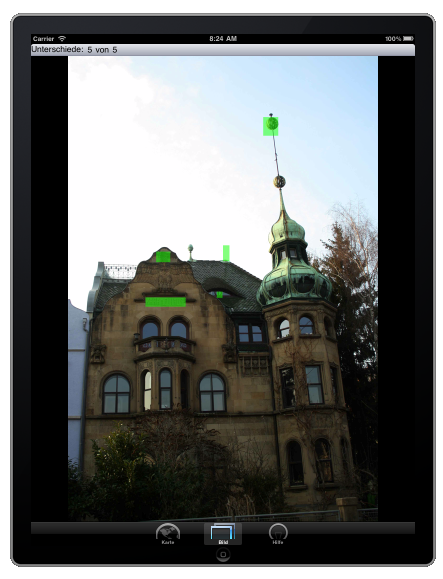
\includegraphics[width=1.0\textwidth]{bilder/loesung3.png}
  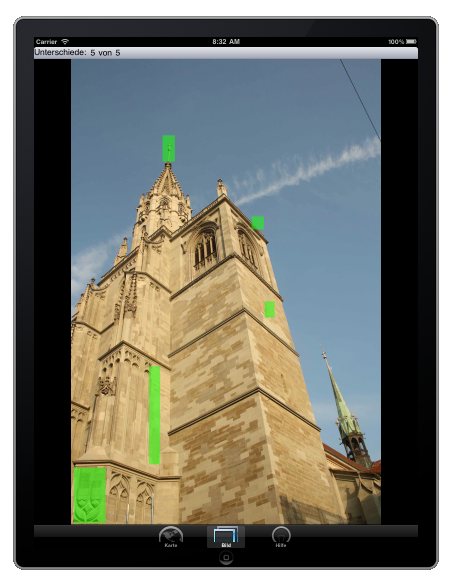
\includegraphics[width=1.0\textwidth]{bilder/loesung4.png}
  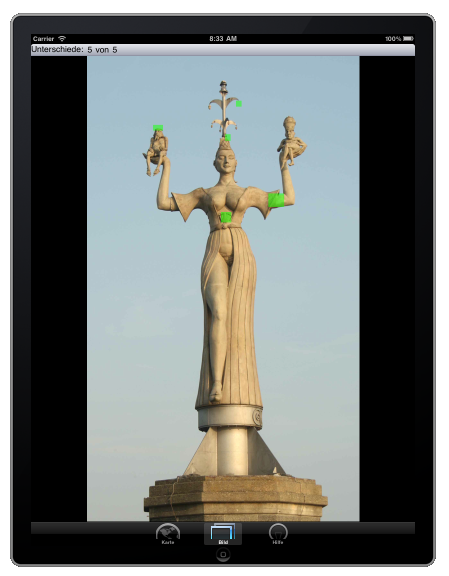
\includegraphics[width=1.0\textwidth]{bilder/loesung5.png}
          	
		\newpage	

	
 
	%Quellvz
	\begin{thebibliography}{99}
			\bibitem{x}Titel, Autor\\
			http://www.example.com\\
			Stand: 17.03.2010	
			
			
					
	\end{thebibliography} 
		
	
\end{document}